\documentclass[11pt,oneside,letterpaper]{article}

% graphicx package, useful for including eps and pdf graphics
\usepackage{graphicx}
\usepackage{grffile}
\usepackage{subfig}
%\DeclareGraphicsExtensions{.pdf,.png,.jpg}

% basic packages
\usepackage{color}
\usepackage{parskip}
\usepackage{float}
\usepackage{microtype}
\usepackage{url}
\urlstyle{same}

\usepackage[hidelinks]{hyperref}
\hypersetup{colorlinks=true,linkcolor=black,citecolor=black,urlcolor=black}

\usepackage{longtable}
\usepackage[]{algorithm2e}

% reference figures across documents
% \usepackage{xr}
% \externaldocument{mers-structure_supp}

% text layout
\usepackage{geometry}
\geometry{textwidth=15cm} % 15.25cm for single-space, 16.25cm for double-space
\geometry{textheight=22cm} % 22cm for single-space, 22.5cm for double-space

% helps to keep figures from being orphaned on a page by themselves
\renewcommand{\topfraction}{0.85}
\renewcommand{\textfraction}{0.1}

% bold the 'Figure #' in the caption and separate it with a period
% Captions will be left justified
\usepackage[labelfont=bf,labelsep=period,font=small]{caption}

% review layout with double-spacing
%\usepackage{setspace}
%\doublespacing
%\captionsetup{labelfont=bf,labelsep=period,font=doublespacing}

% cite package, to clean up citations in the main text. Do not remove.
%\usepackage{cite}
\usepackage{natbib}
%\renewcommand\citepleft{(}
%\renewcommand\citepright{)}
%\renewcommand\citepform[1]{\textsl{#1}}

\usepackage{amsmath}

%\usepackage{lineno}
%\linenumbers

% Remove brackets from numbering in list of References
%\renewcommand\refname{\large References}
%\makeatletter
%\renewcommand{\@biblabel}[1]{\quad#1.}
%\makeatother

\usepackage{authblk}
\renewcommand\Authands{ \& }
\renewcommand\Authfont{\normalsize \bf}
\renewcommand\Affilfont{\small \normalfont}
\makeatletter
\renewcommand\AB@affilsepx{, \protect\Affilfont}
\makeatother

% comments
%\usepackage{ulem}
\definecolor{purple}{rgb}{0.459,0.109,0.538}
\def\tb#1#2{\sout{#1} \textcolor{purple}{#2}}
\def\tbc#1{\textcolor{purple}{[#1]}}
\def\gdc#1{\textcolor{blue}{[#1]}}
\def\lmc#1{\textcolor{green}{[#1]}}

% symbols
% \newcommand{\chiSq}{\chi^{2}_{df}} %LM: ancient DNA? =P %GD: quite :)
% \newcommand{\dtmrca}{\Delta_\mathrm{TMRCA}}
% \newcommand{\undtmrca}{\delta_\mathrm{TMRCA}}
% \newcommand{\dspr}{d_\mathrm{SPR}}

%%% TITLE %%%
\title{\vspace{1.0cm} \LARGE \bf TITLE HERE}

\author[1,2]{Sidney Bell}
\author[3]{Leah Katzelnick}
\author[1]{Trevor Bedford}

\affil[1]{Vaccine and Infectious Disease Division, Fred Hutchinson Cancer Research Center, Seattle, WA, USA}
\affil[2]{Molecular and Cell Biology Graduate Program, University of Washington, Seattle, WA, USA}
\affil[3]{Some Department, University of California, Berkeley, CA, USA}

% \date{\today}

\begin{document}
\maketitle

\begin{abstract}
  % SB: Placeholder copied over from epidemics abstract
  Dengue virus (DENV), the causative agent of dengue hemorrhagic fever, exists as four genetically distinct serotypes, DENV1-4.
  These serotypes are antigenically distinct: symptomatic reinfection with a homotypic virus is very rare, while reinfection with a heterotypic virus is associated with severe disease.
  Until recently, it has been assumed that viruses within each serotype are antigenically uniform.
  However, specific genotypes of each serotype have been anecdotally associated with varying severity of patient outcomes and epidemic magnitude.
  One hypothesis is that each serotype contains overlooked, meaningful antigenic diversity.
  Here, we analyze a publically available neutralization titer dataset to quantify and identify genetic drivers of DENV intraserotype antigenic diversity.
  We map antigenic changes to specific branches of the virus phylogeny, and interpolate across the tree to estimate the antigenic distance between pairs of viruses based on their relative positions in the phylogeny.
  We report modest but significant antigenic diversity within each serotype of DENV, suggesting that antigenic interactions between specific viral genotypes meaningfully contributes to DENV epidemiology.
  In real-world virus populations, even subtle shifts in antigenic phenotypes—below the limit of detection in neutralization assays—can contribute to viral fitness and drive clade turnover.
  To characterize these more nuanced antigenic changes, we also analyze DENV population dynamics.
  We estimate the strength of selection for novel epitopes across the viral phylogeny and characterize patterns of competition between co-circulating DENV genotypes.
  By leveraging both molecular data and real-world population dynamics, these results provide a more nuanced understanding of dengue antigenic evolution, with important ramifications for improving vaccine design and epidemic preparedness.

\end{abstract}

\pagebreak

\section*{Introduction}

Dengue virus (DENV), the causative agent of dengue hemorrhagic fever (DHF), is a mosquito-borne flavivirus that exists as four genetically and antigenically distinct serotypes, DENV1-4.
Although each serotype of DENV was independently introduced to human populations X-X years ago, recent globalization has led to cocirculation of multiple serotypes in many tropical areas, and most individuals living in hyperdemic areas will experience multiple DENV infections over their lifetime.
Primary infections are typically mild, and confer lifelong homotypic protection and temporary heterotypic protection.
As this heterotypic immune response wanes, however, remaining cross-reactive antibodies may bind--but not neutralize--an infecting heterotypic virus, leading to serious infection for some individuals via antibody dependent enhancement (ADE).
In total, DENV causes ~X fatalities each year, most of which are the result of these immune-mediated interactions between different serotypes of DENV.

Notably, each serotype also contains a substantial amount of genetic diversity, with viruses in each serotype differing by X-X\% at the amino acid level in the E protein (the predominant target of the neutralizing antibodies).
Moreover, observational evidence suggests that specific strains--within each serotype--can influence case outcomes and epidemic magnitude.
Katzelnick et al. recently generated a dataset to test the hypothesis that specific strains within each serotype are antigenically distinct from one another.
Antigenic distinctness between a "reference virus" and a "test virus" is experimentally measured using a neutralization titer, which measures how well sera drawn after infection with the reference virus is able to neutralize the test virus in vitro.
A high titer value represents stronger cross-neutralization and smaller antigenic distance between the two viruses.
To measure the pairwise antigenic distances for a panel of X strains of DENV, Katzelnick et al. infected naive non-human primates with each virus, drew sera at 3 months post-infection, and then titered this sera against each virus in the panel.
Importantly, they found that some sera neutralized heterotypic viruses better than it neutralized homotypic viruses.
This was true for sera from non-human primates, Nicaraguan children, and vaccine recipients, which suggests that each serotype of DENV contains at least some antigenic diversity.
However, it is not understood how this antigenic diversity maps to DENV genetic diversity and evolution.
It is also unknown whether this intraserotype antigenic diversity meaningfully impacts DENV population dynamics and epidemic patterns.

Here, we build upon this analysis to characterize the mechanistic relationship between DENV genetic and antigenic evolution.
We also investigate the extent to which antigenic novelty, both between and within serotypes, drives DENV population dynamics and clade turnover.
In doing so, we hope to better inform epidemic preparedness and dengue vaccine design efforts.



\section*{Results}
\subsection*{DENV antigenic relationships are roughly symmetrical and track DENV genetic relationships}
Generally, pairs of DENV strains that are more genetically distinct are also more antigenically distinct  (Figure~\ref{genetic_antigenic_distance}), but the high dimensionality of these pairwise comparisons makes this relationship difficult to interpret.
\begin{figure}[h]
 \centering
	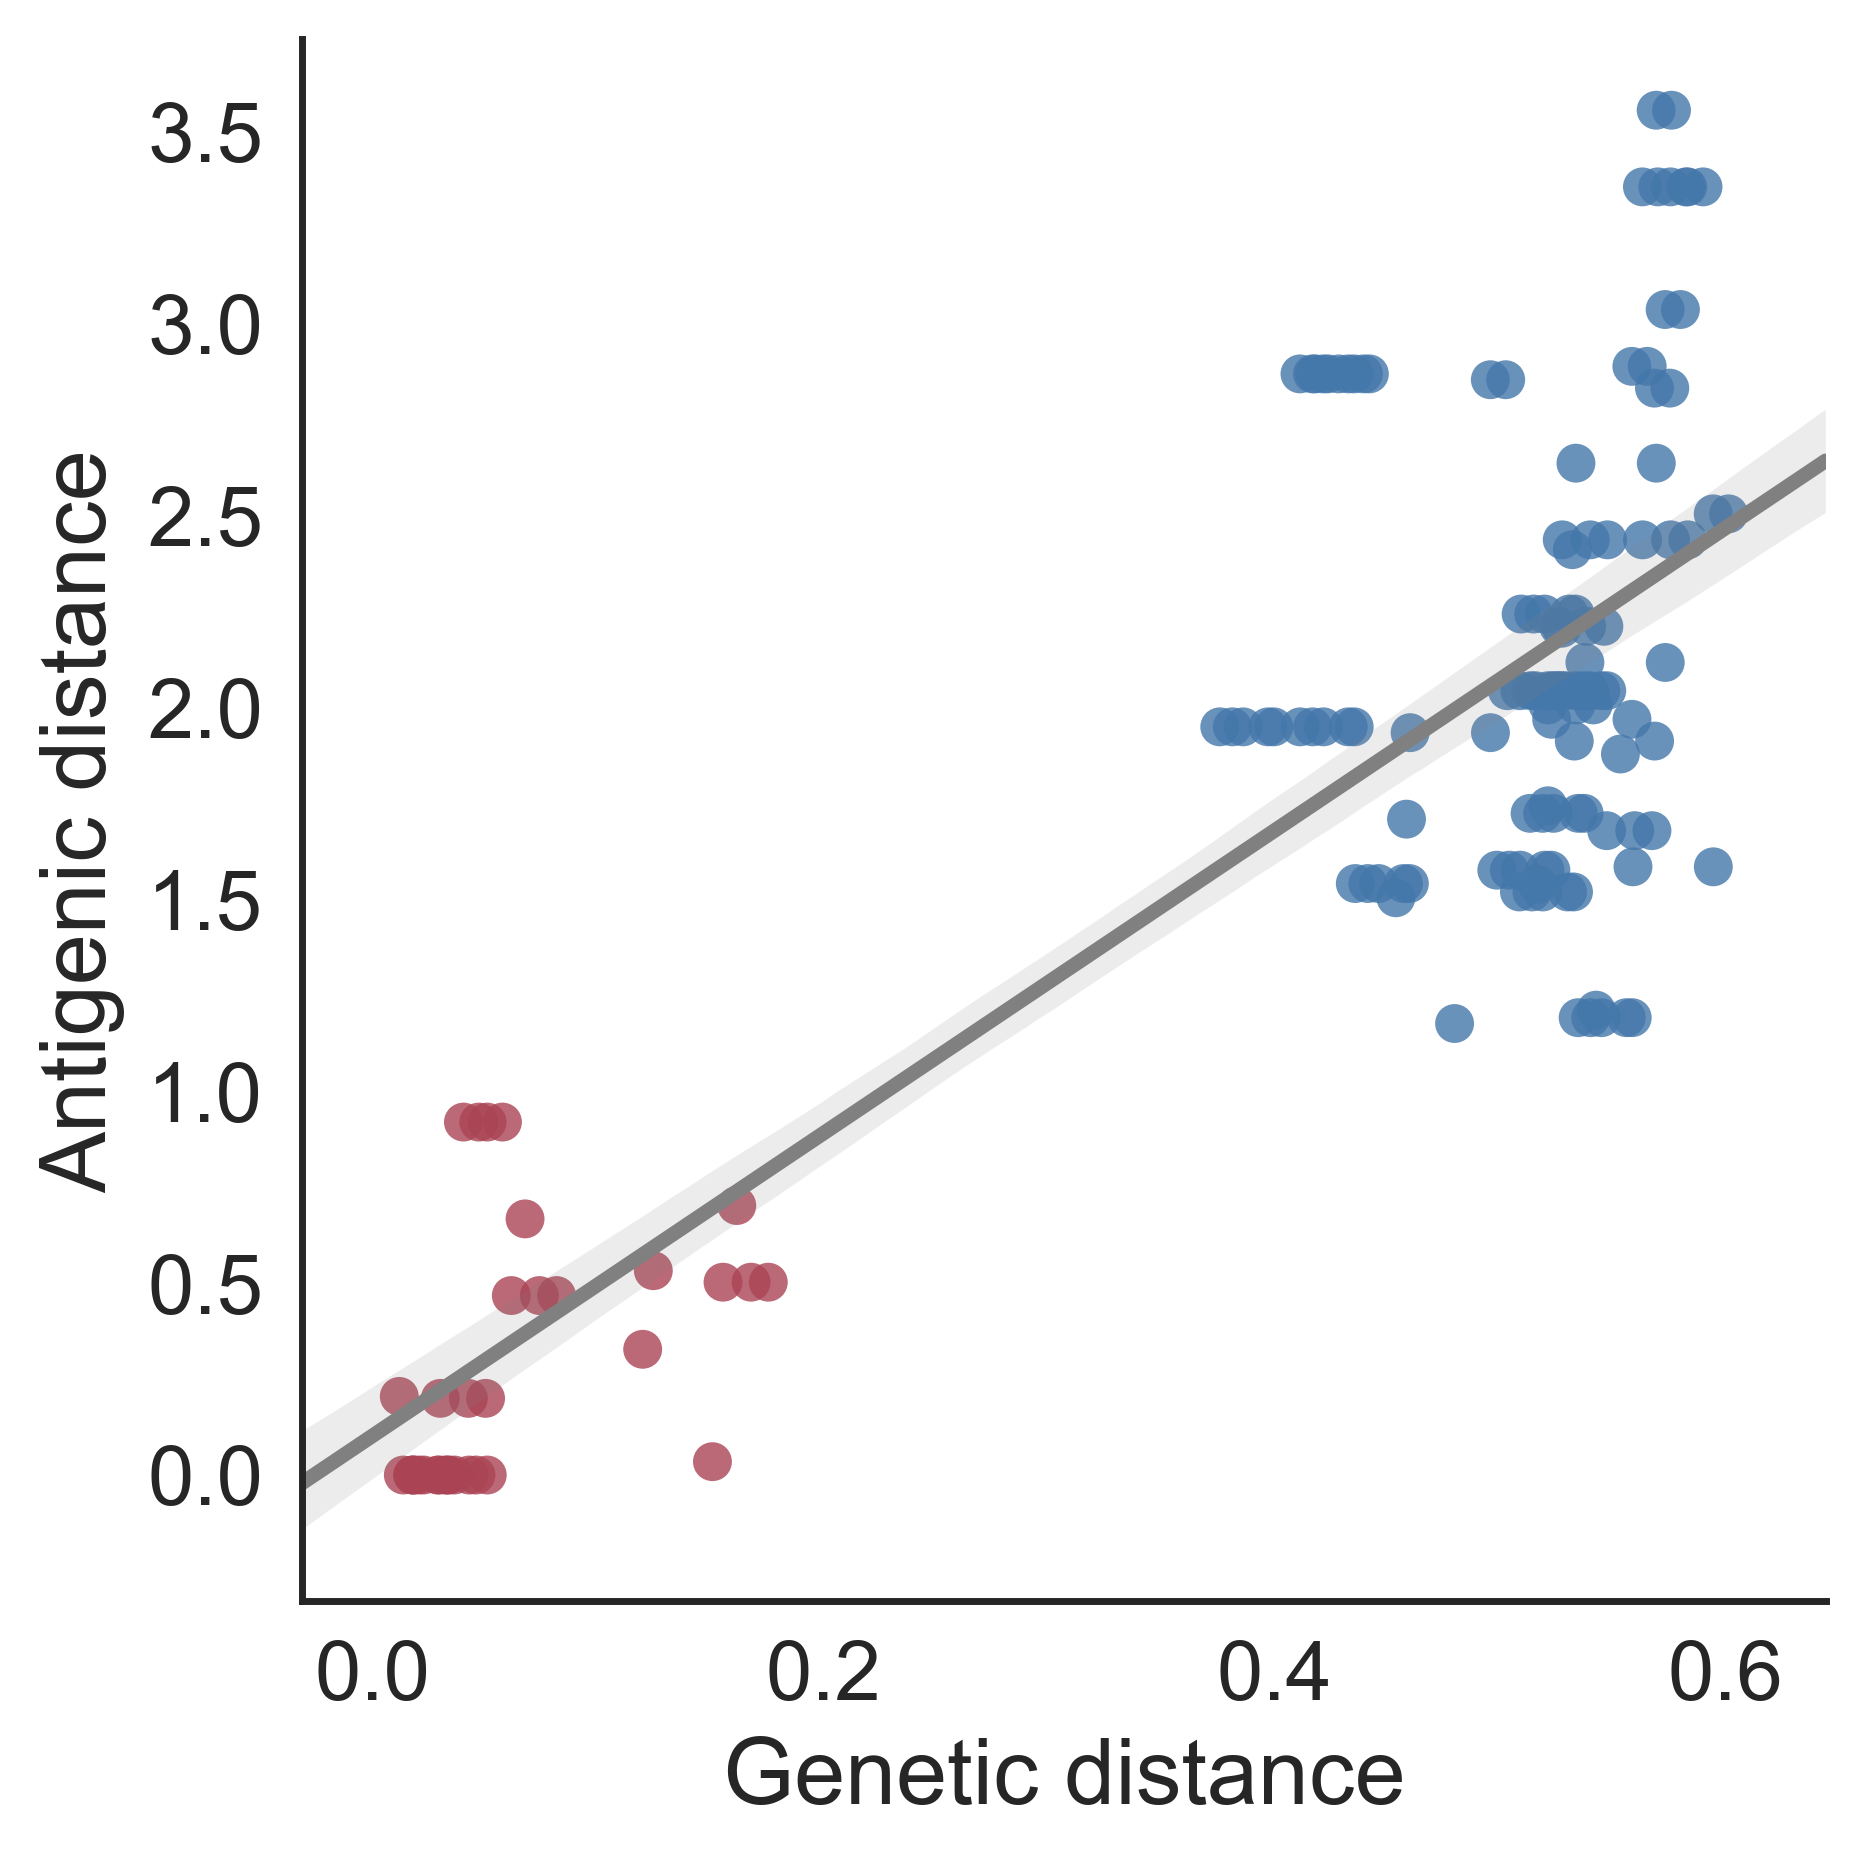
\includegraphics[width=0.40\textwidth]{figs/genetic_antigenic_distance.png}
	\caption{\textbf{
Genetic distance is generally correlated with antigenic distance between pairs of canonical dengue clades.
  }}
	\label{genetic_antigenic_distance}
\end{figure}
Phylogenies are a familiar tool for understanding many pairwise genetic distances between viruses; similarly, we can use a phylogenetics-based model to understand pairwise antigenic distances between viruses.
We adapted an established phylogenetics-based model of antigenic evolution; this model, referred to as the "tree model", is described in detail in %\cite_p{Neher_PNAS_2016}.
This model describes how the relative positions of viruses $i$ and $j$ on the phylogeny relate to the antigenic distance between them.

We assembled a dataset that included the X strains used in Katzelnick et al., as well as a selection of all publicly available DENV sequences: we preferentially included full-genome sequences from primary isolates, and subsampled a maximum of X sequences per region, per month, from 1970 - present (N = X).
We then built a maximum-likelihood phylogenetic tree to establish the genetic relationships among the isolates.
To estimate the antigenic relationships between the isolates, we needed to quantify how much antigenic change, denoted $d_b$, occurred along each branch, $b$, in the viral phylogeny.
Importantly, quantifying $d_b$ for each branch allows us to estimate the antigenic distance between any two viruses in the tree, $i$ and $j$, based on their relative positions in the phylogeny.
This corresponds to the sum of $d_b$ for each branch $b$ along the path from $i$ to $j$ in the phylogeny:
$$\hat{T}_{ij} \propto \sum_{b} d_b$$
Notably, though, some virus and sera samples show greater binding avidity than others overall.
As in Neher et al., we also correct for these virus avidities $v_i$ and serum potencies $p_j$.
Our final titer estimation is thus calculated as: $$T_{ij} \approx \hat{T}_{ij} = \sum_{b} d_b + v_i + p_j$$

Each of these parameters, $d_b$, $v_a$, and $p_j$, is inferred such that our predicted titers most closely match the measured titers for each pair of viruses in the training data set (a randomly selected subset of the available titer measurements).
In doing so, we make a few assumptions to promote biologically reasonable parameter values.
First, we encourage a parsimonious explanation of antigenic change, wherein most branches in the phylogeny do not contribute to antigenic change, by using L1 regularization (akin to placing an exponential prior) on values of $d_b$.
This means that most values of $d_b$ are 0.
We also assume that antigenic change is symmetrical and additive, and thus each branch is assigned only one, non-negative value of $d_b >= 0$.
Indeed, once we correct for the overall binding avidities of each virus and serum sample ($v_i$ and $p_j$, respectively), most titers are roughly symmetric: the distribution of $T_{ij} - T{ji}$ is symmetrical and centered at X, with a standard deviation approaching the WORD of the assay %(Figure~\ref{titer_symmetry}).
% \begin{figure}[h]
%  \centering
% 	\includegraphics[width=0.75\textwidth]{./figs/titer_symmetry.png}
% 	\caption{\textbf{
% Pairwise titers are roughly symmetrical once overall virus avidity and serum potency are corrected for.
% }
% 	\label{titer_symmetry}
% \end{figure}
We thus assume that $v_a$ and $p_b$ are normally distributed, and use L2 regularization (akin to placing a Gaussian prior) on values of $v_a$ and $p_b$.
We ultimately infer the values of $d_b$, $v_i$ and $p_j$ that minimize the objective function $C = things$ for each virus $i$ and serum $j$ in the training data set.
We then assess model performance based on how well the trained model is able to predict a withheld/unseen random subset (test set) of the data.
By testing how well our model and inferred parameter values are able to predict these unseen values, we can quantify how sufficiently this model of antigenic evolution explains the observed changes in antigenic phenotype.

\subsection*{DENV antigenic phenotypes are clade-specific}
We can use this framework to test two hypotheses by making small changes to the model.
Our null hypothesis is that all of the viruses within each serotype of DENV are antigenically uniform.
This is expressed mathematically by only allowing branches of the tree that lie between serotypes to take non-zero values of $d_b$.
The test error for this model then quantifies how much of the observed antigenic variation is unexplained by serotype-level relationships alone.

\begin{figure}[h]
 \centering
	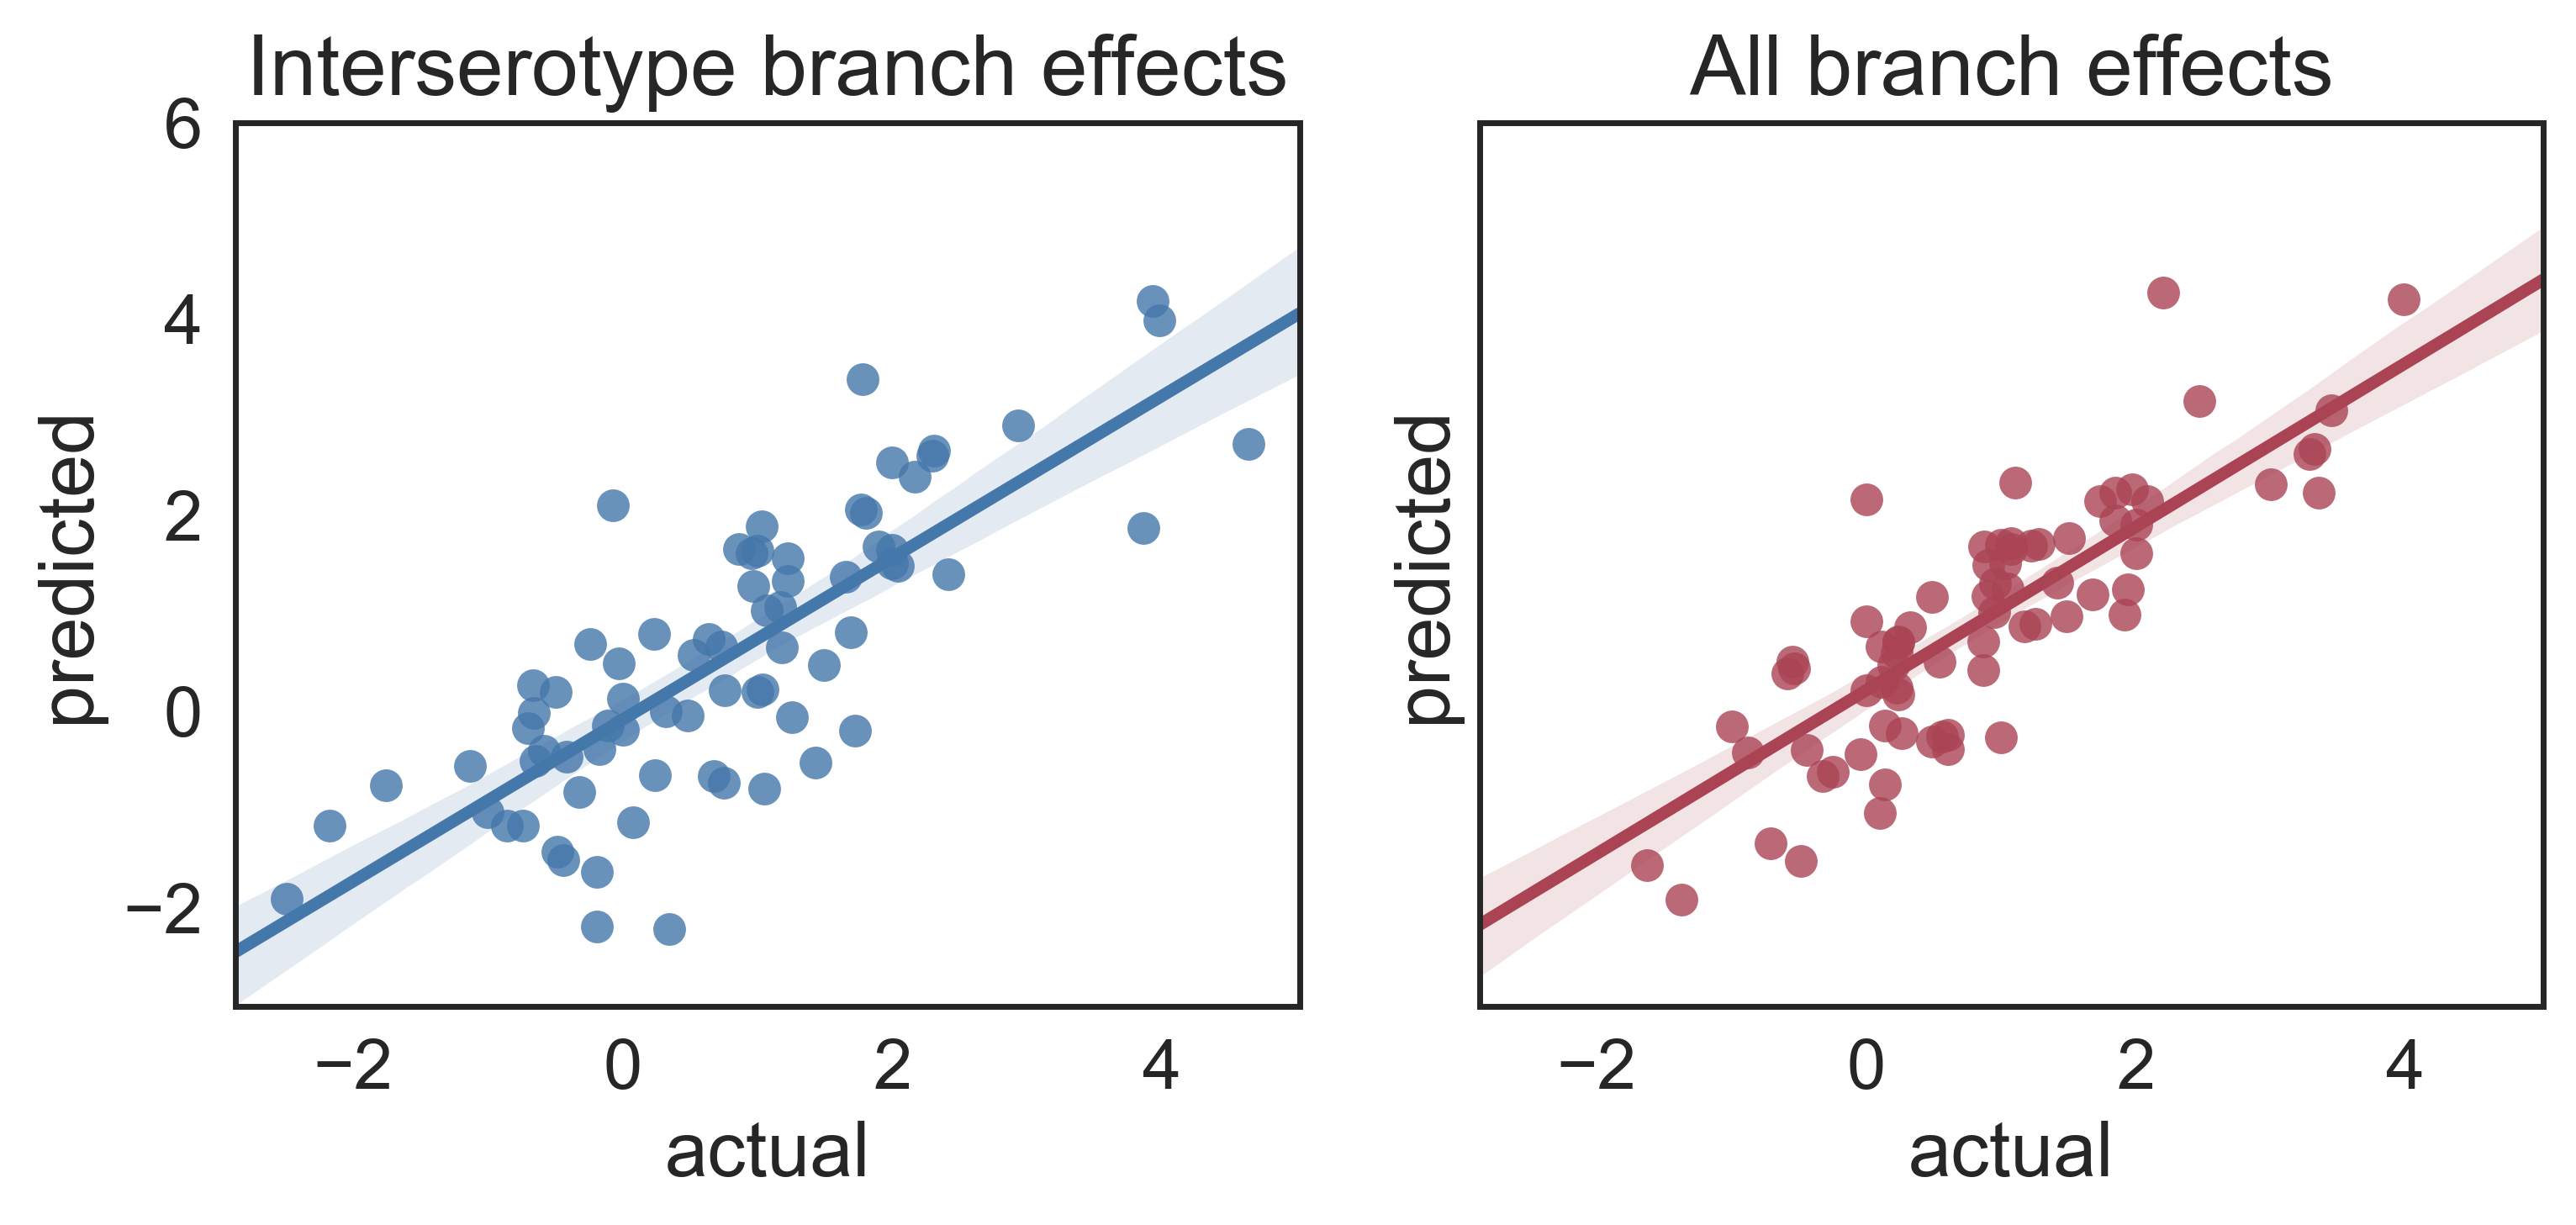
\includegraphics[width=0.75\textwidth]{figs/test_error.png}
	\caption{\textbf{
Within-serotype variation significantly contributes to dengue antigenic phenotypes.
}}
	\label{test_error}
\end{figure}

We find that these coarse-grained interserotype antigenic relationships are able to explain most of the observed antigenic variation, and the model performs well in cross-validation: the root mean squared test error (RMSE) is X, indicating that serotype-level relationships alone are able to predict most titers within one two-fold titer drop (Figure~\ref{test_error}).
This is similar to how well this model performs on influenza data, and to how well the original analysis from Katzelnick et al. described this data.

Although this null hypothesis explains most of the observed variation in DENV antigenic phenotypes, we also wanted to test the alternative hypothesis that each serotype of DENV contains significant antigenic variation.
This is expressed mathematically by allowing any branch in the tree to contribute to DENV antigenic evolution.
We find that including these within-serotype effects substantially lowers our test RMSE to X, indicating that within-serotype variation is necessary to accurately describe DENV antigenic evolution (Figure~\ref{test_error}).

\subsection*{There are at least X distinct antigenic phenotypes of DENV}
\begin{figure}[h]
 \centering
	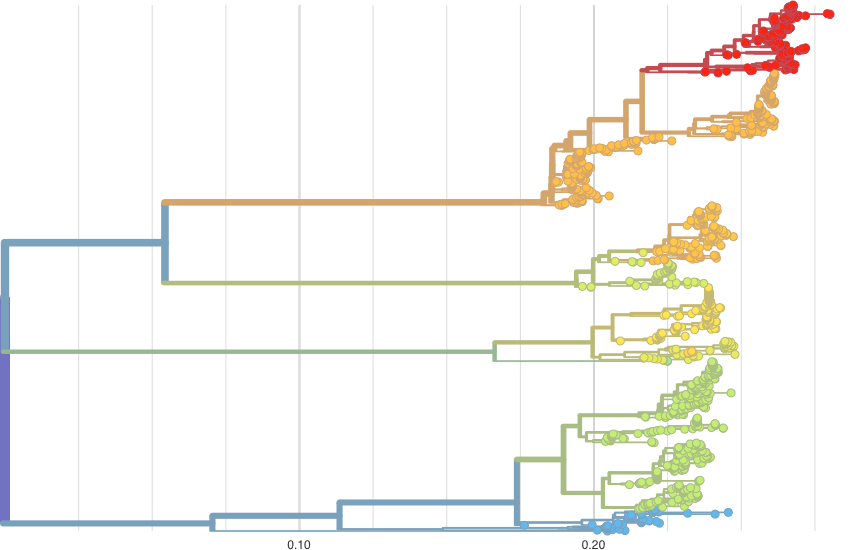
\includegraphics[width=0.75\textwidth]{figs/tree.png}
	\caption{\textbf{
Each serotype of dengue contains at least X distinct antigenic phenotypes.
}}
	\label{tree}
\end{figure}

Titer measurements are extremely labor intensive.
As a result, our results are limited by the resolution available in publicly accessible data, and represent a lower-bound on the antigenic diversity within DENV.
Nevertheless, we identify at least X antigenically distinct clades of DENV that are at least X log2 titer units apart in antigenic space from the nearest clade.
Figure~\ref{tree} illustrates measured titers and inferred antigenic distances across the viral phylogeny, and these results are available in full for exploration at http://www.nextstrain.org/dengue.
Importantly, each serotype of DENV contains X-X of these distinct antigenic phenotypes.

\subsection*{Antigenic novelty contributes to DENV viral fitness}

As a viral strain circulates through a population, viral fitness declines over time as more hosts become immune.
If a new viral strain enters this population, its success will be partially determined by its ability to escape this pre-existing immunity.
Antigenically novel strains, or strains that are more antigenically distant from previously circulating viruses, are thus more antigenically fit.
Antigenically driven selection leads to clade turnover as as antigenically novel strains increase in frequency and antigenically stale strains die out.

The strength of antigenically driven selection, and its impact on viral population dynamics, depends on the breadth of antigenic phenotypes displayed.
For example, influenza A displays an exceptionally broad range of antigenic phenotypes that are distinct enough from one another to enable immune escape.
This makes antigenic novelty a strong driver of influenza population dynamics.
Contrastingly, measles displays only one antigenic phenotype.
Antigenic novelty does not contribute to measles population dynamics.

We find strong evidence for antigenic heterogeneity within dengue serotypes.
Within each serotype, however, we observe relatively small antigenic distances between canonical genotypes (mean = X-fold) and antigenically distinct clades (mean = X-fold).
We wanted to quantify the impact of this observed antigenic heterogeneity on real-world dengue population dynamics.

To do so, we adapt a simple deterministic model from REF to directly quantify dengue antigenic fitness and its impact on clade turnover.
We model the relative antigenic fitness of dengue clade $i$ at time $t$ ($f_i(t)$), as a function of population immunity to $i$--or the proportion of the population that is nonsusceptible to strain $i$--at time $t$, denoted $P_i(t)$.
We estimate population immunity, $P_i(t)$, as a function of the antigenic distance between $i$ and each non-overlapping clade $j$ (denoted $D_{ij}$), weighted by the number of years since exposure, $n$, and the relative frequency of $j$, $x_j(t-n)$.
Mathematically, this is expressed as: $$ f_i(t) = 1. - P_i(t)$$
$$P_i(t) = \sum_{n=1}^{n=N} (w(n)  \sum_{j} x_j(t-n) * C( D_{ij})) $$
Where $w(n)$ represents the waning of immunity over time, and $C(D_{ij})$ represents the probability of protection against $i$ given prior exposure to $j$ (both simple linear transformations; see methods).

We can then use these estimates of viral fitness to predict relative clade growth and decline, :
$$\frac{\hat{x_i}(t+N)}{x_i(t)} = e^{x_i(t) \beta f_i(t)}$$



However, although DENV clades turn over every X-X years on average in hyperendemic populations, with serotypes switching every X-X years (Figure~\ref{frequencies_time}), it is not understood whether these dynamics are driven by neutral stochastic turnover and seasonal bottlenecking or by population immunity and viral antigenic novelty.

\begin{figure}[h]
 \centering
	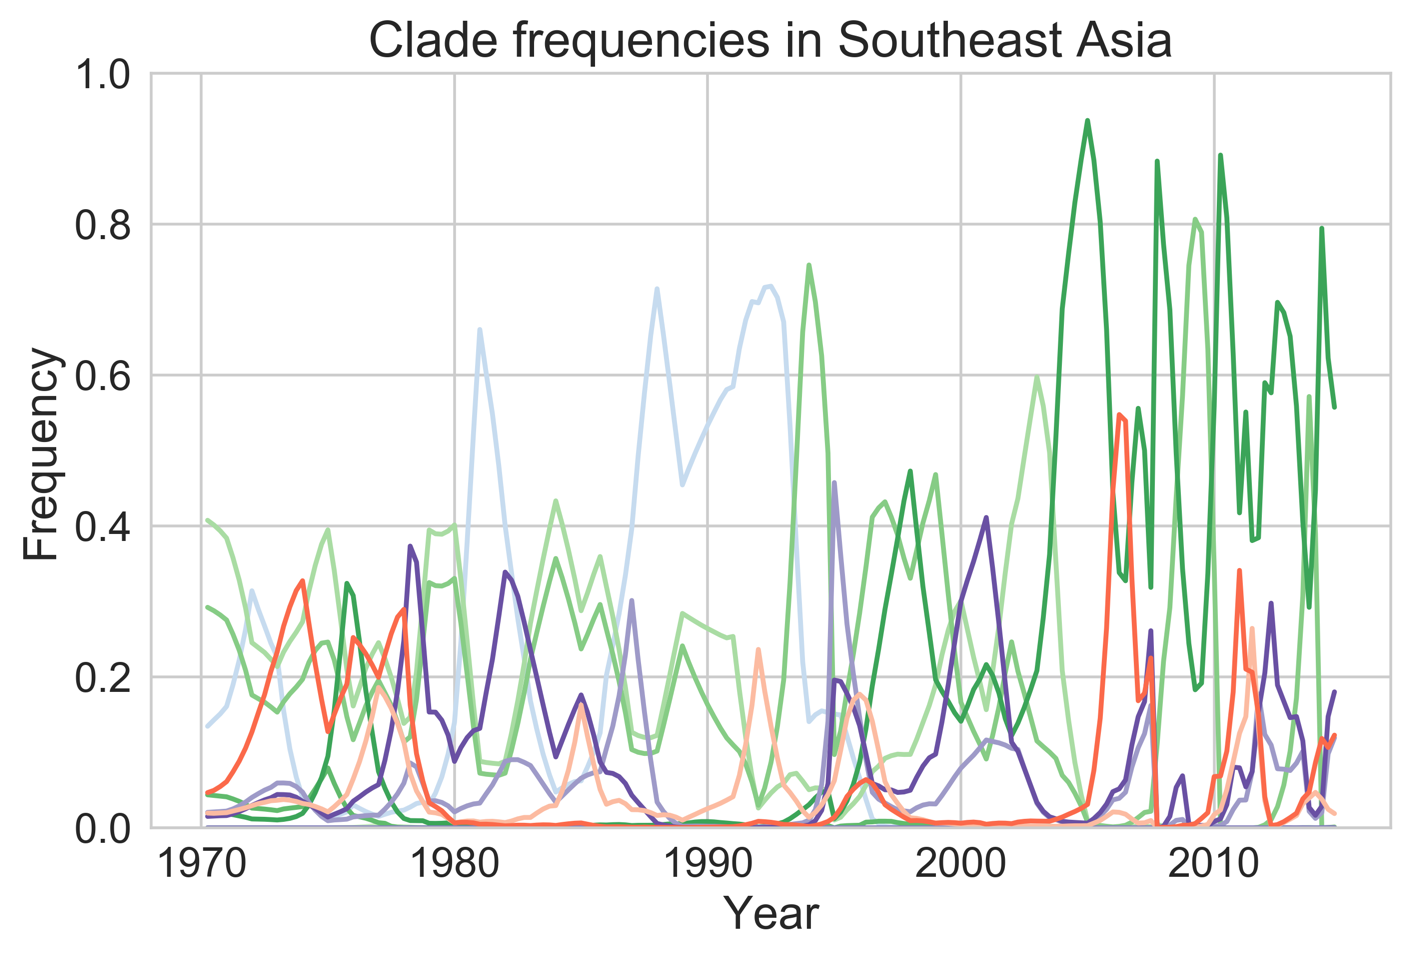
\includegraphics[width=0.75\textwidth]{figs/frequencies_time.png}
	\caption{\textbf{
Dengue clades turn over every X-X years in southeast asia
}}
	\label{frequencies_time}
\end{figure}

Understanding how antigenic phenotypes contribute to viral population dynamics has important applications for epidemic surveillance and vaccine design.
We hypothesize that antigenically novel strains of DENV are better able to escape population immunity, thereby gaining access to more susceptible individuals and outcompeting the incumbent strains to rise in population frequency.

To test this hypothesis, we adapt a model of viral antigenic fitness originally developed by Luksza and Lassig, wherein antigenically novel clades are expected to grow over the next X years, and antigenically stale clades are expected to die out.
Antigenic novelty of clade $i$ is quantified as $1 - P_i(t)$, where $P_i$ is the proportion of the population that is immune to clade $i$ at time $t$.
$P_i(t)$ is estimated as the frequency-weighted antigenic distance between clade $i$ and each clade $j$ that has circulated in the past $X$ seasons:  $$P_i(t) = \sum{n=1}^{n=X} \gamma(n) \sum{j} x_j(t-n) C(T_ij)$$
As described earlier, $T_{ij}$ is estimated as $\hat{T_{ij}} = \sum{b} d_b$, using the $d_b$ values inferred by either the interserotype-only or full-tree model of DENV antigenic evolution.
Based on results from <katzelnick et al pnas 2017>, we assume that a titer against strain $i$ of $T_i$ is linearly related to $C_i$, the  probability that this individual will be protected from severe infection when exposed to strain $i$.
We assume that titers wane over time according to a linear function, $\gamma(n)$.

How much antigenic novelty contributes to DENV fitness can be quantified by how well estimates of population immunity, under each model of dengue antigenic evolution, predicts the relative change in frequency for each strain: $$\hat{x_i(t+5)/x_i(t)} \approx \hat{x_i(t+5)/x_i(t)} \propto e^x_i(t) * P_i(t)$$

\begin{figure}[h]
 \centering
	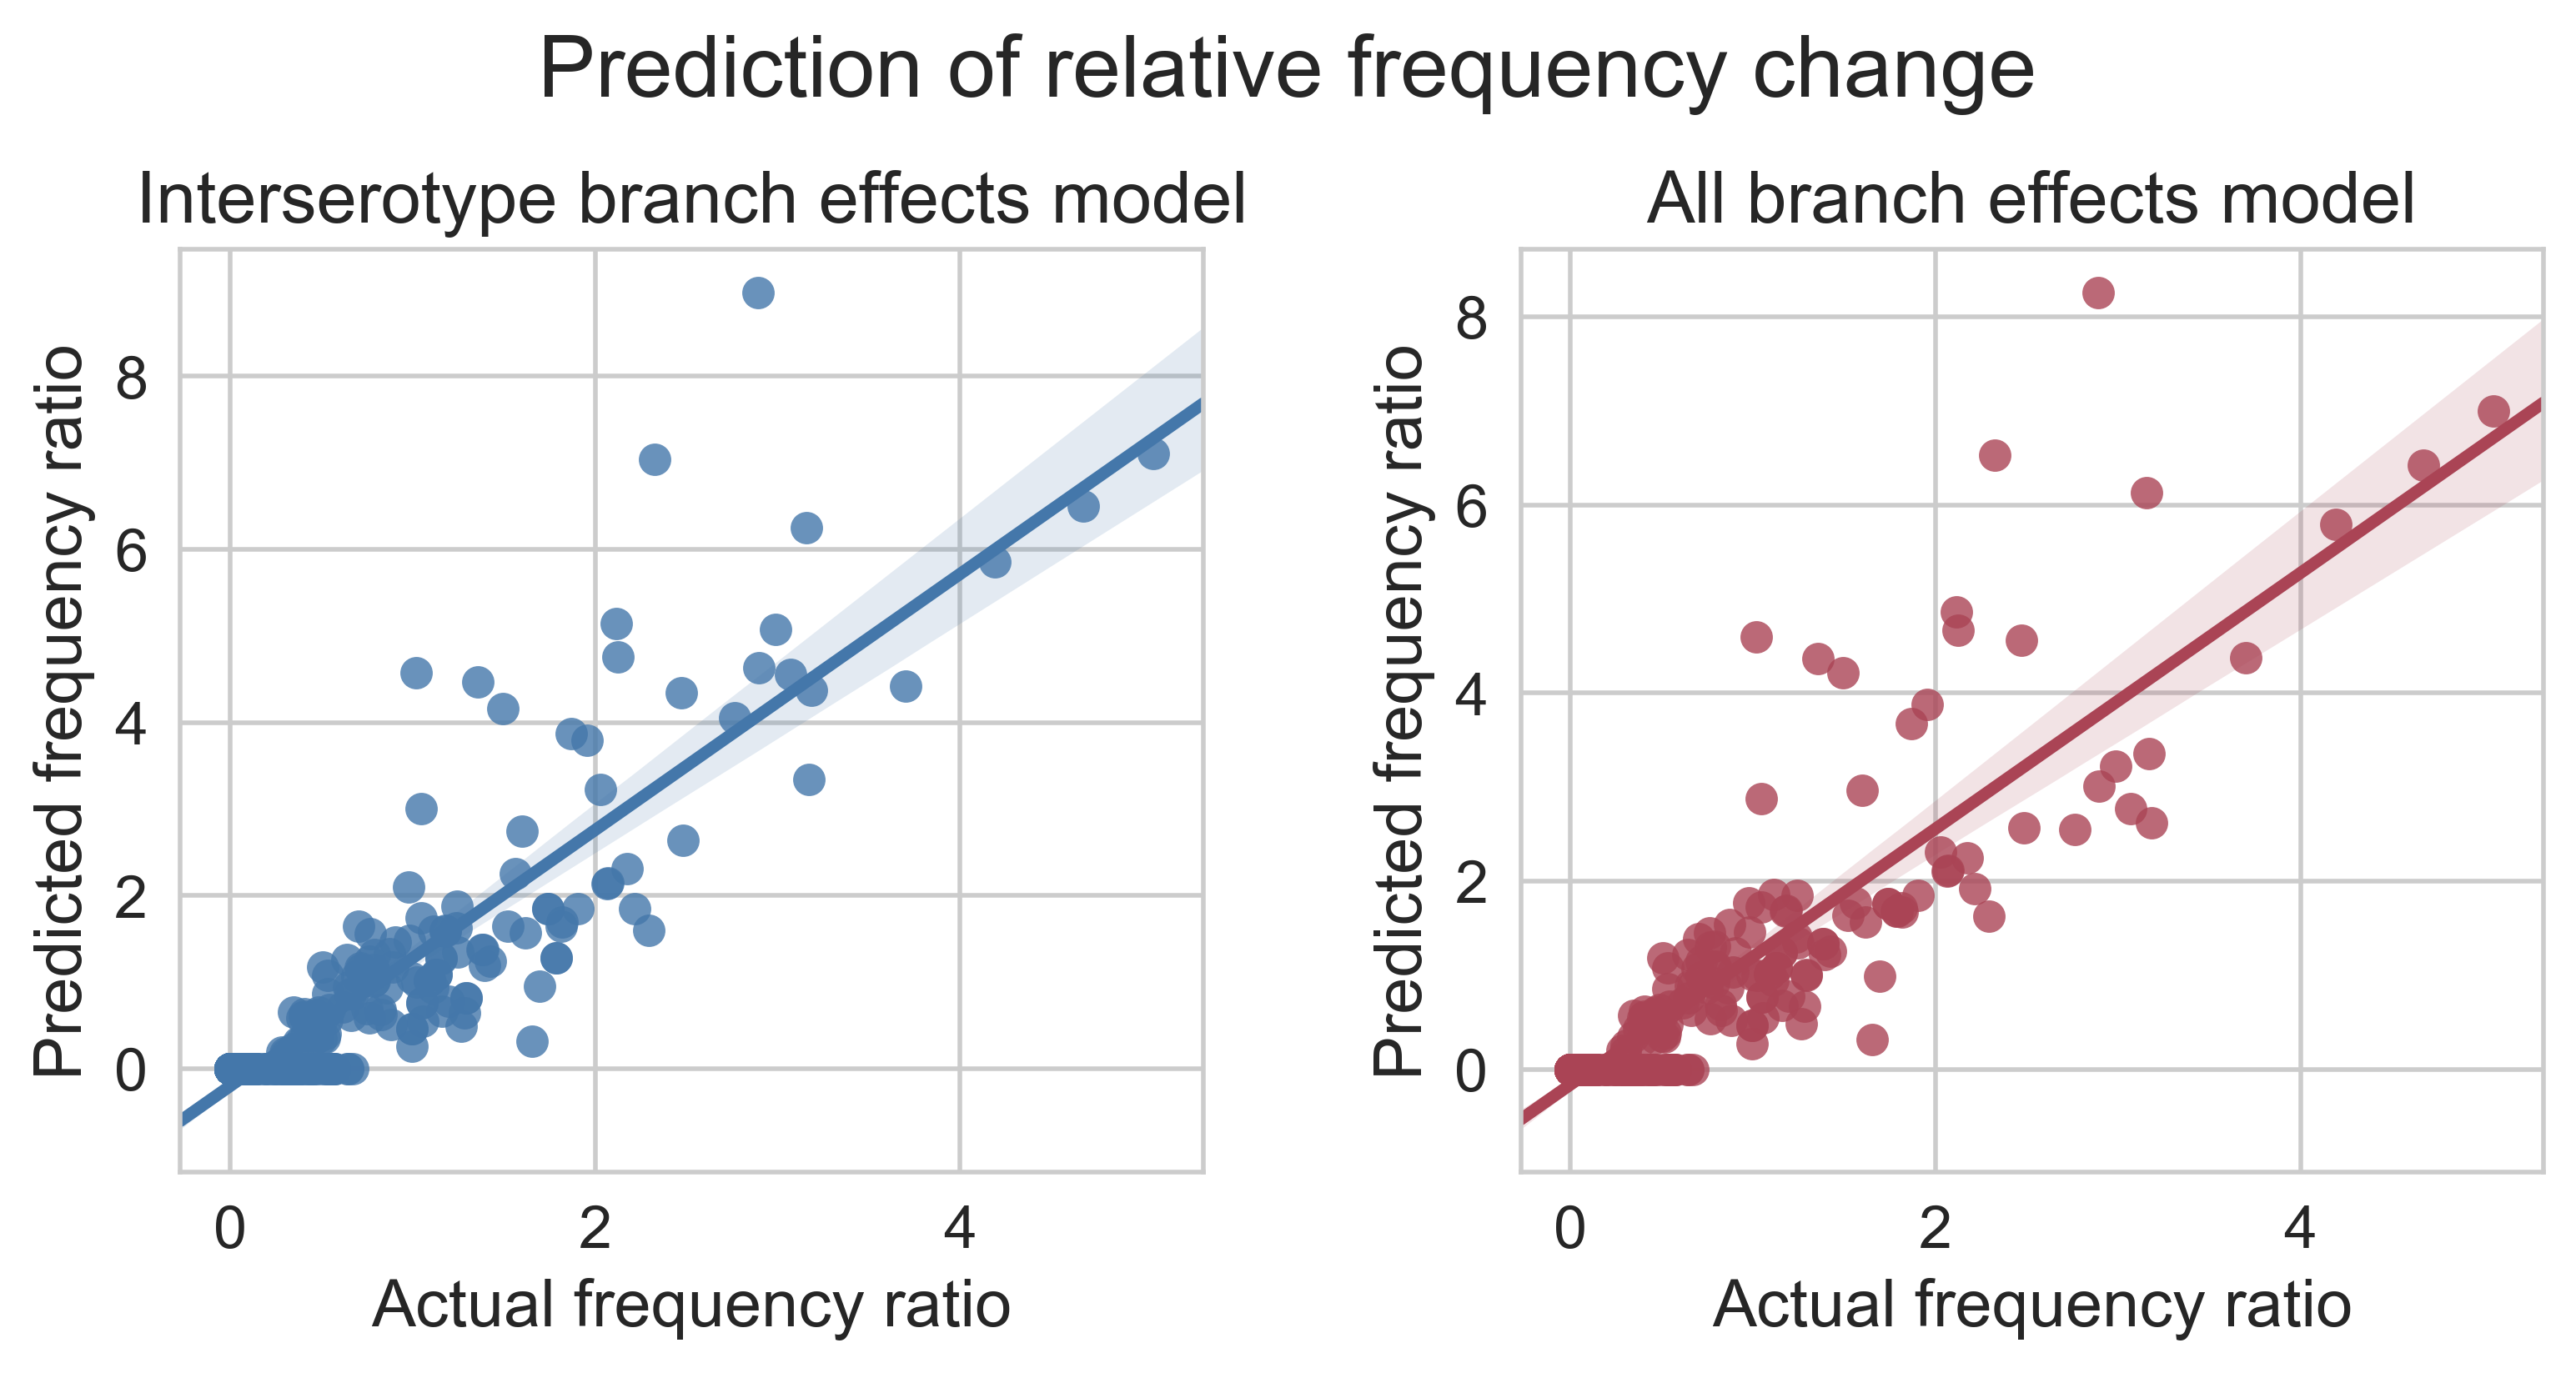
\includegraphics[width=0.75\textwidth]{figs/frequency_predictions.png}
	\caption{\textbf{
Antigenic novelty drives dengue clade turnover.
}}
	\label{frequency_predictions}
\end{figure}

When we treat all strains as antigenically uniform (where all values of $T_{ij} = 0$), we are unable to predict strain frequency (RMSE = X, Figure~\ref{frequency_predictions}).
However, we find that the serotype-level antigenic relationships (using values of $T_{ij}$ from the "interserotype model" above) are able to explain X of the observed change in population frequency (Figure~\ref{frequency_predictions}), indicating that antigenic novelty is an important driver of dengue clade turnover.

\subsection*{DENV population dynamics are putatively shaped by serotype-level relationships}
To assess the extent to which subtler within-serotype antigenic variation contributes to DENV clade turnover, we repeated the analysis from  using clade-specific values of $T_{ij}$ from our "full tree model" above.
Curiously, although we find good support for the biological reality of these antigenic differences within each serotype, we find that they do not improve our predictions of population dynamics beyond coarse serotype-level designations (Figure~\ref{frequency_predictions}).
This could be because XYZQ (see discussion).

%(Figure~\ref{FIGURE1_LABEL_HERE})

\section*{Discussion}
Our results show that each serotype of DENV contains multiple distinct antigenic phenotypes. We also find that DENV antigenic evolution is driven by DENV genetic evolution, and meaningfully contributes to DENV viral fitness. However, this intraserotype antigenic heterogeneity does not appear to drive dengue clade turnover.

\subsection*{Strengths and limitations of the model}
As discussed more extensively in Neher et al, the tree model makes two major implicit assumptions.
First, the model assumes that titers are symmetric (i.e., that $T_{ij} \approx T_{ji}$).
As shown in Figure \ref{titer_symmetry}, this is largely accurate: once overall virus and sera potency are accounted for, titers are roughly symmetric after a primary infection.
It has been previously hypothesized that the order in which populations are exposed to different serotypes and/or genotypes of DENV was an important driver of outbreak severity.
The finding that titers are roughly symmetrical--i.e., that $T_{ij} \approx T_{ji}$, once the overall viral avidity is accounted for--suggests that epidemic magnitude is instead driven by a combination of population demography, the time between epidemics, and the antigenic distance between strains $i$ and $j$, rather than the order in which they appear in the population.
While this is a subtle distinction, it has important ramifications for assessing epidemic risk.

The model also assumes that antigenic change is additive (i.e., that as viruses diverge genetically, they are also "pushed" apart in antigenic space, rather than pulled closer together).
For most viruses, this assumption holds true except for instances where a single site is independently mutated along multiple branches.
For DENV, however, it has been hypothesized that enhanced infection via ADE is a fitness advantage.
ADE only occurs when viruses share partially overlapping immune profiles: viruses that are very near in antigenic space are cross-neutralized, and viruses that are very far in antigenic space are not recognized by the cross-reactive antibodies required for ADE.
Thus, it has been hypothesized that DENV fitness is optimized by a moderate amount of antigenic novelty, suggesting that its antigenic evolution is driven by both a "push" to escape neutralization and a "pull" towards more cross-reactive antigenic phenotypes.
The additive formulation of the tree model inherently only incorporates the former.
And yet, despite this constraint, the model predicts out-of-sample titers with accuracy near the level of error inherent in the assay.
We speculate that this is an artefact of the fact that this dataset does not incorporate the effects of ADE -- the "pull" that the tree model does not capture.
It is striking, then, that this divergence-based model of antigenic evolution is still strongly predictive of DENV clade success.
It is unclear whether this is because ADE does not contribute to DENV viral fitness, or XYZQ.

\subsection*{Strengths and limitations of the data}
Due to the sparcity of available techniques and sera samples, DENV antigenic relationships are incredibly challenging and costly to measure accurately.
DENV neutralization titer measurements are inherently noisy due to substantial host heterogeneity and the dynamic nature of the virion structure.
Additionally, although ADE is an important component of DENV antigenic relationships and evolution, it is very difficult to measure due to technical barriers precluding the use of an FC-$\gamma$ receptor bearing cell lines.
Finally, there is no ideal model of DENV infection; while the non-human primates used to generate these data likely recaptilate relevant antibody responses, they do not recapitulate the full disease progression to DHF.
Ultimately, titer measurements may not precisely indicate antigenic distance.

Nevertheless, there are many pieces of evidence--both in the literature and in our current study--that suggest these data are incredibly valuable and relevant for understanding DENV antigenic relationships.
In their original publication, Katzelnick et al elegantly showed that although these are noisy measurements, the same overall relationships between viruses can be observed in sera from non-human primates, children, and vaccine recipients.
Furthermore, titer values obtained on mosquito cells and on X cells were well-correlated.
This suggests that although titer measurements are noisy, these values do faithfully represent the relative antigenic distances between DENV viruses in human antigenic space.
This is further supported by recent analysis by Katzelnick et al. of longitudinal cohort data, which showed that PRNT50 titers, like those used here, are good predictors of case outcomes in an endemic setting.
Additionally, our results show that antigenic distances based on titer measurements are able to predict real-world viral population dynamics.
This suggests that although PRNT50 titers are imperfect approximations of antigenic distance, they have sufficient information content to predict outcomes for both individuals and populations.

\subsection*{These results represent a lower-bound on DENV intraserotype antigenic heterogeneity}
This dataset is by far the most comprehensive available: the available measurements span the full geographic and temporal range of DENV evolution, but they are generally limited to one strain per canonical DENV "genotype".
Thus, while our results clearly show that genotypes within a serotype are significantly antigenically diverse, we are unable to assess the extent of antigenic diversity among strains within these genotypes.
However, we find that DENV antigenic evolution tracks DENV genetic evolution, with each X sub/site in E conferring approximately X log2 titer units of distance in antigenic space.
Given that each serotype of DENV contains between X-X subs/site of genetic diversity in E, and the measured and interpolated antigenic relationships reported here span X-X units within a serotype, we expect that these results represent a lower-bound on the amount of antigenic heterogeneity present within each serotype of DENV.
Thus, we expect that increased resolution, as more data becomes available, will show antigenic distances between genotypes of similar magnitude, but with greater within-genotype heterogeneity.

\subsection*{Antigenic novelty drives DENV serotype replacement}
Increased data availability may also shed light on why we do not detect sub-serotype levels of antigenic novelty contributing to viral fitness.
We find that in Southeast Asia, serotype dominance switches on average every X-X years; clade dominance switches every X-X years.
We find that serotype-level antigenic novelty contributes to DENV fitness, but clade-level antigenic novelty putatively does not.
This raises the question of why, then, we observe relatively frequency clade turnover, and whether antigenic novelty contributes to this process.
We propose three hypotheses as potential explanations.
First, it is entirely possible that sub-serotype antigenic differences are not large enough to influence viral fitness.
Second, given more complete data, we may be able to detect more fine-grained antigenic differences that better explain the observed population dynamics.
Finally, this may be a function of demography.
Naive individuals are equally susceptible to all DENV strains, and thus do not contribute to the antigenic fitness of any particular strain.
Individuals who have had exactly one infection are differentially susceptible to different DENV strains, and thus increase or decrease particular strains' antigenic fitness in that population.
The average time between primary and secondary infection in Southeast Asia is X.
We would thus expect that clade dynamics driven by post-primary individuals would play out over a period of ~X years, which is substantially shorter than the observed period of serotype turnover.
% some actual hypothesis here? i.e., how does boosting in post-secondary individuals play into this?

\subsection*{Implications for DENV clade designations}
Appropriately classifying evolving pathogens into clades is important for promoting a common language and defining relevant experimental conditions for researchers.
DENV viruses are typically classified into "genotypes" originally named by either Twiddy and Holmes or SOMEONE.
These designations were comprehensive at the time they were proposed, but as DENV continues to emerge as a global pathogen, most of these canonical genotypes have extensively diversified.
For example, the canonical genotype X (denoted with * in Figure \ref{tree}), now contains X clades that are separated by BRANCHLENGTH, comparable to the BRANCHLENGTH separating "genotype X" from "genotype Y".
Our results also show that each of these canonical genotypes represents a distinct antigenic phenotype; while we cannot comment on the antigenic diversity within each genotype, we expect that our current results represent a substantial underestimation of antigenic heterogeneity.
Initially, we propose a classification schema of X (illustrated in Figure SOMETHING), based on X.
This proposed classification schema better represents the genetic diversity of DENV, although it does not fully represent the antigenic diversity of DENV.

\subsection*{Opportunities for enhanced surveillance and epidemic preparedness}
This study represents proof of concept for both predicting DENV antigenic phenotypes based on sequence data, and then using this phenotypic data to predict which DENV clades will dominate in the coming season.
Recent analysis of a longitudinal cohort study in Nicaragua suggests that for individuals, the risk of severe infection is driven by their titers before their secondary infection.
We hypothesize that population-level epidemic severity is similarly dependent on population exposure history and antigenic distance.
Obtaining additional titer data describing the antigenic phenotypes of each distinct circulating clade could enable robust predictions of epidemic severity, improving resource allocation and epidemic preparedness.
We thus urge surveillance agencies to invest in routine antigenic characterization of circulating DENV clades.

\subsection*{Implications for vaccine design and opportunities for future investigation}
% I need to think about what to put here.

\newpage

\section*{Methods}
\subsection*{METHODS SUBSECTION 1 TITLE HERE}

METHODS SECTION 1 TEXT HERE.

\begin{equation}
\mathrm{Pr}(j | R_{0}, \omega) = \frac{\Gamma(\omega j+j-1)}{\Gamma(\omega j) \, \Gamma(j+1)} \; \frac{(\frac{R_{0}}{\omega})^{j-1}}{(1+\frac{R_{0}}{\omega})^{\omega j+j-1}}.
\label{EQ1_REF_NAME}
\end{equation}

Hey look there's math stuff in Equation \ref{EQ1_REF_NAME}

% \begin{algorithm}[H]
%  \KwData{Array of case cluster sizes in outbreak $\mathbf{c} = (c_1, c_2, \ldots, c_K)$, sequences available $M$, total outbreak size $N$, where $N = \sum_{i=1}^{K} c_{i}$.}
%  \KwResult{Array of sequence cluster sizes sampled: $\mathbf{s} = (s_1, s_2, \ldots, s_K)$.}
%  Draw $s_i$ from a hypergeometric distribution with $c_i$ successes, $N-c_i$ failures after $M$ trials\;
%  \While{$i < K$}{
%   $i = i + 1$\;
%   $M = M - s_{i-1}$\;
%   Compute the probability mass function (pmf) for all possible values of $s_i$, $\mathbf{p} = (p(0)^{\mathrm{bias}}, p(1)^{\mathrm{bias}}, \ldots, p(c_i)^{\mathrm{bias}}) \times (\sum_i p_i^{\text{bias}}) ^{-1}$, where $p(\cdot)$ is the pmf for a hypergeometric distribution with $c_i$ successes, $N-c_i$ failures after $M$ trials\;
%   Draw a sequence cluster size $s_i$ from array of potential sequence cluster sizes $(0, 1, \ldots, c_i)$ according to $\boldsymbol p$\;
%  }
%  Add remaining sequences to last sequence cluster $c_K = M - s_{K-1}$\;
%  \caption{\textbf{Multivariate hypergeometric sampling scheme.}
%  Pseudocode describes the multivariate hypergeometric sampling scheme that simulates sequencing.
%  Probability of sequencing a given number of cases from a case cluster depends on cluster size and sequences left (\textit{i.e.}\ ``sequencing capacity'').
%  The bias parameter determines how probability mass function of the hypergeometric distribution is concentrated.
%  }
%  \label{hypergeometric}
% \end{algorithm}

\subsection*{Data availability}
Sequence data and all analytical code is publicly available at \href{https://github.com/blab/structured-mers}{github.com/blab/structured-mers}.

\section*{Acknowledgements}
We would like to thank Allison Black for useful discussion and advice.
GD is supported by the Mahan postdoctoral fellowship from the Fred Hutchinson Cancer Research Center.
TB is a Pew Biomedical Scholar and is supported by NIH R35 GM119774-01.
AR was supported in part by the European Union Seventh Framework Programme for research, technological development and demonstration under Grant Agreement no. 278433-PREDEMICS and no. 725422-RESERVOIRDOCS, and the Wellcome Trust through project 206298/Z/17/Z.

We gratefully acknowledge the contribution of the following scientists for sharing MERS-CoV sequence data before publication:

First M.\ Surname$^{1}$

$^{1}$Person 1 is here \\

% \bibliographystyle{mbe}
% \bibliography{mers-structure}

\newpage

% SUPPLEMENT STARTS HERE

\setcounter{figure}{0}
\setcounter{table}{0}
\renewcommand{\thefigure}{S\arabic{figure}}
\renewcommand{\thetable}{S\arabic{table}}

\begin{longtable}{ | r | l | p{2cm} | l | l | } % COLUMN FORMATS

  \caption{TABLE CAPTION HERE} \label{TABLE LABEL HERE} \\
  \endfirsthead

  1 & KSA-378 & KJ713296 & camel & 2013-11 \\
  2 & KSA-363 & KJ713298 & camel & 2013-11 \\
  3 & KSA-503 & KJ713297 & camel & 2013-11 \\

\end{longtable}

\begin{figure}[h]
\centering
	% \includegraphics[width=0.65\textwidth]{figures/mers_exploded.png}
	\caption{\textbf{SUP FIGURE 1 TITLE }
SUPP FIGURE 1 CAPTION
	}
	\label{SUP_FIGURE_1_LABEL}
\end{figure}

% EXTRA TEXT SNIPPET BANK

% map the relationship between DENV genetic changes, defined as branches on the viral phylogeny, to changes in dengue antigenic phenotype, defined as drops in titer measurements.
%
% * phylogenies consist of a topology and distances, described as branch lengths.
% When using the phylogeny to describe antigenic distances instead of genetic distances, we take the topology directly from the virus sequence tree.
% We then essentially re-optimize the branch lengths (expressed as Db) such that they best explain all of the observed pairwise antigenic relationships.
% * each branch gets a Db value that represents the amount of antigenic change on that branch.
% * <what that would look like with only three viruses / one measurement>
% * we can then predict antigenic relationships between any two viruses based solely on their relative positions in the phylogeny.
% *
% * because we need to represent many such pairwise measurements, Db values across the tree are inferred such that they minimize the mean squared error between
%
%
% SOMETHING limited by the sparcity of available data, we are able to confidently place a lower bound on the extent of antigenic heterogeneity within each serotype.
% To investigate the extent to which these



% There are several implicit assumptions in this model.
% First, because entirely naive individuals, as well as those who have experienced at least two infections, are uniformly susceptible or protected from severe disease, we focus our analysis on the window of time between primary and secondary infections.
% In hyperendemic areas, this is approximately X years.
% As cross-protective titers wane on a similar time scale, we ignore population demography in quanitfying population immunity.

% We ultimately quantify population immunity to strain $i$, the probabiliy that a random individual in the population is susceptible to strain $i$ at time $t$, as: $$P_i(t) = STUFF$$


\end{document}
